\documentclass[10pt,a4paper]{article}
\usepackage[utf8]{inputenc}
\usepackage[german]{babel}
\usepackage[T1]{fontenc}
\usepackage{amsmath}
\usepackage{amsfonts}
\usepackage{amssymb}
\usepackage{graphicx}
\author{Manuel Rickli, Lukas Stöckli, Michael Plüss}
\title{LED Bank}
\begin{document}
\maketitle

\section{Einleitung}

Das Ziel unserer Gruppe war, eine LED Bank zu bauen. Diese besteht aus 48x8 grünen LEDs, welche als Pixel fungieren. Die LED Bank soll sich mit dem Internet verbinden können und Pixel Daten von dort entnehmen und anzeigen können. Was auch möglich sein soll, ist, einfach kurze Texte anzuzeigen und von rechts nach links scrollen zu lassen.\\
Die Vision ist, diese LED Bank im Zimmer aufhängen oder hinstellen zu können und darauf verschiedenste Informationen darstellen zu können. Ursprünglich waren Anwendungen wie eine Uhr oder eine Wetterangabe geplant, oder sogar kleine 48x8 Pixel Filmchen.\\
Es gibt mehrere Gründe, weshalb wir uns vorrangig für eine zweidimensionale LED Konstellation entschieden haben, anstatt für eine dreidimensionale. Einerseits können wir so gewohnt konventionell Text darstellen und zweitens versprachen wir uns davon eine wesentlich einfachere Verdrahtung. Das Hauptproblem so viele LEDs überhaupt mit dem Arduino anzusteuern haben wir so aber nicht umgangen.\\

\section{Hauptteil}

\subsection{Umsetzung}

\subsubsection{Display}

!!!!!!!!!!!!!!!!!!!!!!!!!!!!!!!!!! TODO!!!!!\\
(Bild)\\\\

Die 384 LEDs befinden sich verteilt auf zwei Steckbrettern. Die acht Reihen der Bank werden direkt vom Arduino angesprochen. Die 48 Kolonnen steuern wir über drei Pins des Arduinos mittels Shift Registern. Ein Shift Register hat jeweils acht Output Pins, weshalb wir insgesamt sechs Shift Register benutzen, welche in Reihe geschaltet sind.\\
Wir erreichen die Darstellung eines komplexen Pixelmusters, indem wir jeweils einen Pin bei den acht Reihen einschalten und die anderen ausschalten und dann die Pixeldaten der Zeile in die Shift Register einfüttern. So wird jeweils eine horizontale Linie dargestellt. Diese lassen wir einen kurzen Moment leuchten und gehen dann zur nächsten Zeile über. Wenn wir alle Zeilen dargestellt haben, haben wir ein Frame 'gezeichnet'. Mit einer genug schnellen Taktrate ist das so entstehende Flimmern auch kein grosses Problem mehr.\\

\subsubsection{Code}

Der Code für das Arduino haben wir in der Arduino IDE geschrieben und bildet die Kontrolle über den Display, sowie die Kommunikationsstelle zum Internet.\\
Um Texte darstellen zu können haben wir viele Bitmuster für die einzelnen Buchstaben einprogrammiert, welche auf unsere Bedüftnisse angepasst sind.\\

\subsubsection{Webseite}

Auf dem Arduino läuft ein kleiner Webserver, der eine Konsole zur Verfügung stellt. Der Server schickt dem Client HTML Code, den der Browser dann in die sichtbare Website umwandelt. Über ein Eingabefeld kann Text an den Server übergeben werden, der dann auf der LED-Matrix angezeigt wird. Über Knöpfe können Requests für das Wetter und die Uhrzeit ausgeführt werden, dessen Resultat dann ebenfalls angezeigt wird.

\subsection{technische Details}

\subsubsection{Display}

Wir haben für unsere Anzeige folgende Bauteile verwendet:

\begin{itemize}
\item LED 20mA, 2,2V
\item Widerstand 3.3k$\Omega$
\item Widerstand 220$\Omega$
\item Schieberegister 74HC595
\item Transistor Array ULN2803
\item Kondensator 1$\mu$F
\end{itemize}

Da die LED's mit 20mA betrieben werden sollte und  \[R = 5V/20mA = 250\Omega\] haben wir 220$\Omega$ Widerstände als Vorwiderstand eingebaut. Der Strom wäre leicht höher als 20mA, die 5V des Arduino erreichen jedoch auch nicht ganz die Anzeige aufgrund von Spannungsabfall. Diese Vorwiderstände befinden sich zwischen den Schieberegistern und den LED-Kolumnen. Die Reihen werden direkt über das Arduino angesteuert. Da dieses bei den Output-Pins jedoch nur ca. 40mA gesourced oder gesinkt werden können, wird der ULN2803 dazwischen geschaltet. Diesen kann man bis 500mA und 50V betreiben. Davor wird für jede Reihe ein 3.3k$\Omega$ Widerstand geschaltet, da über die Leitungen vom Arduino nur noch Impulse an den ULN2803 gesendet werden, welche diesen dann zum Schalten bringen. Die ganze Energie kommt also direkt von Ground und 5V und nicht über die Arduino Outputs.

Um die Schieberegister anzusteuern benötit man bloss drei Verbindungen zum Arduino:
\begin{itemize}
\item Latch Pin
\item Clock Pin
\item Data Pin
\end{itemize}

Der Clock Pin bestimmt, wann über den Data Pin die Register beschrieben werden. Nur wenn dieser auf HIGH ist, können die im Data Pin gespeicherten Bytes gesendet werden. Ist der Latch Pin auf HIGH, so werden die im Register gespeicherten Reihen mit Spannung versorgt. Deshalb muss vor dem Neubeschreiben dieser auf LOW gesetzt werden. In unserem Falle geben wir mit jedem shiftOut() genau ein Byte mit. Dieses wird immer in dem ersten Register gespeichert. Ist es schon beschrieben, so wird dieses Byte an das nächste Register weitergegeben. Wir rufen also sechs mal shiftOut() auf und geben als erstes Byte die Information für das sechste Register mit.

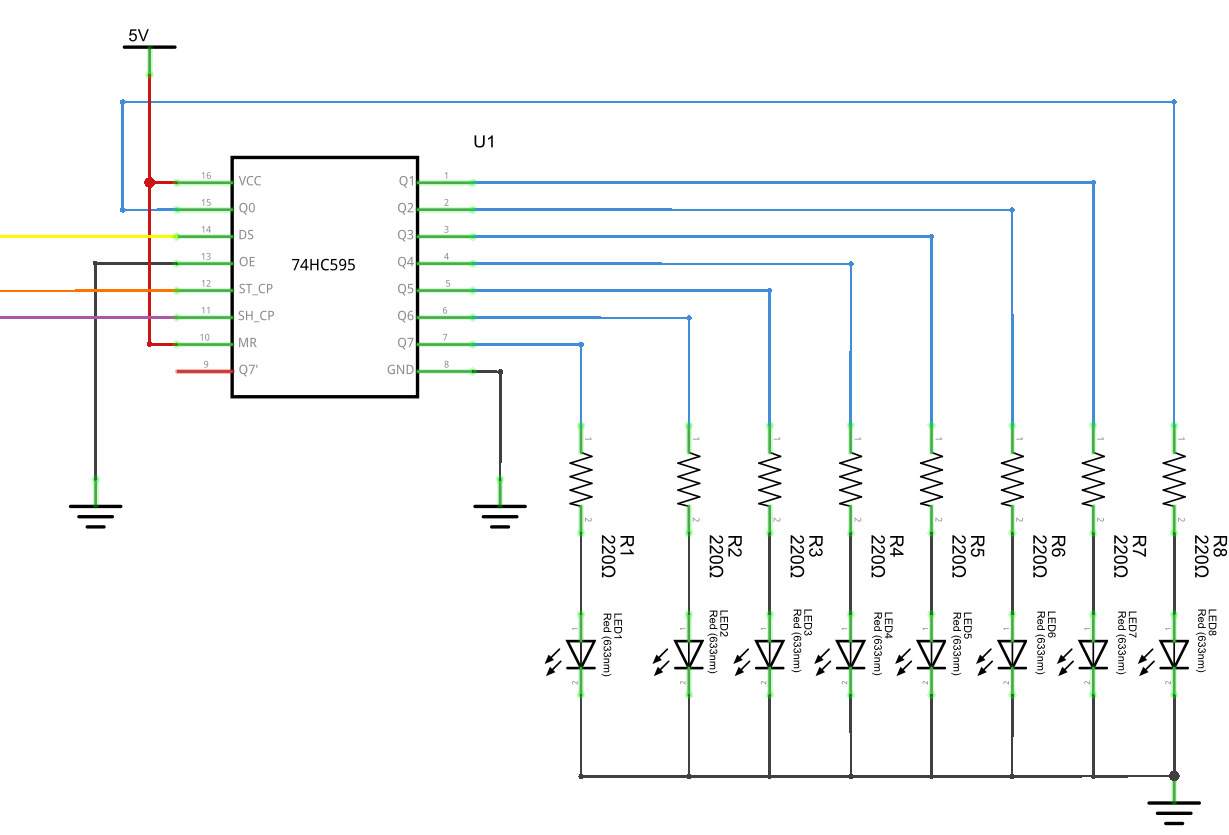
\includegraphics[width=\textwidth]{shiftReg.png}

\subsubsection{Code}

Der Code ist in verschiedene Module unterteilt die zusammen die Funktionalität des Produkts gewährleisten.\\
Das 'main' Modul initialisiert die anderen Module und hält den Mainloop in dem die Frames gezeichnet werden, die Laufschrift geshiftet wird und der Requesthandler arbeitet.\\
Das Modul 'internetInterface' ist verantworlich für die Internetanbindung unseres Systems. Es besteht aus einem Setup-Modul, dass die physische Verbindung initialisiert und den Server startet und dem Requesthandler. Dieser sendet den Code für das Anzeigen der Webseite und bearbeitet die Eingaben über die Console um den Text zu ändern. 
Das Modul 'ledInterface' hält den Grafikspeicher, welcher aus einem 48x8 Char-Array besteht in welchem die Lichtzustände der Pixel gespeichert werden. Es enthält ausserdem die Methoden zur Textbearbeitung. Sie ist verantwortlich für das Übersetzen von Usereingaben in die Bitmap sowie das aktualisieren der Lauftschrift. Hier werden Buchstaben in Arrays mit 8-Bit Zahlen umgewandelt.\\
Das Modul 'chars' hält die ganzen Informationen über die darstellbaren Zeichen. Dies sind einerseits die Bitmap und andererseits die anzuzeigende Breite.\\
Als letztes gibt es das Modul 'ledHardwareControl'. Es ist verantwortlich für die Anzeige des Grafikspeichers auf der LED-Matrix. Über die Pins des Arduinos werden Reihen und Spalten angersprochen um das gewünschte Frame anzuzeigen. Über ein Untermodul werden die Daten reihenweise in die Schieberegister geshiftet.\\

\subsubsection{Webseite}

Auf dem Arduino läuft ein Webserver mit einer Internetseite. Über die IP 192.168.178.42 und Port 80 kann darauf zugegriffen werden. Die Webseite enthält ein Feld um einen neuen Text auf die Anzeige zu laden sowie Buttons um Daten wie Wetter und Uhrzeit anzuzeigen. Der Requesthandler schickt den HTML/CSS Code an den Client. Falls er vom Client einen Request bekommt wird keine Seite gesendet, stattdessen untersucht der Parser die Nachricht und aktualisiert die Anzeige. Falls es sich um das Drücken einer der Buttons handelt, holt sich der Server die Informationen per Request bei der entsprechenden Website. \\

\section{Zusammenfassung}

!!!!!!!!!!!!!!!!!! TODO!!!!!\\
(Wie gut läuft es schlussendlich?)\\

Insgesamt war die LED Bank ein Projekt überschaubarer Komplexität. Darauf hatten wir auch abgezielt. Was schwieriger war als erwartet, war der Umgang mit den Shift Registern, welche sich Anfangs nie so verhalten haben wie wir es geplant hatten. Auch mühsamer als erwartet war die Verbindung des Arduinos mit dem Internet. Die Einschränkung auf Http macht es schwierig auf viele moderne Webseiten zuzugreifen.\\

\section{Quellen}

!!!!!!!!!!!!!!!!!!!!!!!!!!!!!!!!!! TODO!!!!!\\

\end{document}